%%%%%%%%%%%%%%%%%%%%%%%%%%%%%%%%%%%%%%%%%
% fphw Assignment
% LaTeX Template
% Version 1.0 (27/04/2019)
%
% This template originates from:
% https://www.LaTeXTemplates.com
%
% Authors:
% Class by Felipe Portales-Oliva (f.portales.oliva@gmail.com) with template 
% content and modifications by Vel (vel@LaTeXTemplates.com)
%
% Template (this file) License:
% CC BY-NC-SA 3.0 (http://creativecommons.org/licenses/by-nc-sa/3.0/)
%
%%%%%%%%%%%%%%%%%%%%%%%%%%%%%%%%%%%%%%%%%

%----------------------------------------------------------------------------------------
%	PACKAGES AND OTHER DOCUMENT CONFIGURATIONS
%----------------------------------------------------------------------------------------

\documentclass[
	12pt, % Default font size, values between 10pt-12pt are allowed
	%letterpaper, % Uncomment for US letter paper size
	%spanish, % Uncomment for Spanish
	german, % Uncomment for German
]{fphw}

% Template-specific packages

%encoding
%--------------------------------------
\usepackage[utf8]{inputenc}
\usepackage[T1]{fontenc}
%--------------------------------------
 
%German-specific commands
%--------------------------------------
\usepackage[ngerman]{babel}
\usepackage{csquotes}

\usepackage{mathpazo} % Use the Palatino font

\usepackage{graphicx} % Required for including images

\usepackage{booktabs} % Required for better horizontal rules in tables

\usepackage{float} % Floating figures

\usepackage{listings} % Required for insertion of code

\usepackage{enumerate} % To modify the enumerate environment

%----------------------------------------------------------------------------------------
%	ASSIGNMENT INFORMATION
%----------------------------------------------------------------------------------------

\title{Sortieralgorithmen am Gymnasium} % Assignment title

\author{Alexandra Maximova} % Student name

\date{06.05.2020} % Due date

\institute{ETH Zurich \\ Lehrdiplom Informatik} % Institute or school name

\class{Fachdidaktik 2 (Die Erfolgsgeschichte von Computer Science Unplugged)} % Course or class name

\professor{Giovanni Serafini} % Professor or teacher in charge of the assignment

%----------------------------------------------------------------------------------------

\begin{document}

\maketitle % Output the assignment title, created automatically using the information in the custom commands above

%----------------------------------------------------------------------------------------
%	ASSIGNMENT CONTENT
%----------------------------------------------------------------------------------------

\section*{Zielsetzung}
Sortieren wird im Alltag immer mehr vom Rechner übernommen und durch die Suche ersetzt. Dort, wo man früher ein Wörterbuch durchblättern musste und sehr froh war, dass die Wörter darin alphabetisch sortiert sind, kann man heute das gesuchte Wort in ein Suchfeld eingeben und direkt den Eintrag lesen. Früher musste man die eigene Kontaktliste (handgeschrieben auf Papier) durchlesen, um Adressen und Telefonnummern von Freunden zu finden, und war froh, wenn sie einigermassen nach dem ersten Buchstaben vom Namen sortiert waren. Heute die Kontaktliste im eigenen Handy ist immer alphabetisch sortiert, und zusätzlich hat man die Möglichkeit, nach dem Namen zu suchen.

Sortieren und Umsortieren geht blitzschnell, man muss nur auf das richtige Button drucken, und im Nu sind die Einträge nach Datum sortiert; Noch ein Klick -- und sie sind nach Name sortiert. Man hat den Eindruck, dass es automatisch passiert und überhaupt keinen Aufwand braucht.

In diesem Kontext ist es schwierig den SuS zu erklären, warum man überhaupt etwas zu sortieren braucht, wenn man Ctrl+F benutzen kann und viel schneller etwas finden, als ''manuell'' in einer alphabetisch sortierten Vokabelliste.

Ein Ziel dieser Lerneinheit könnte sein, den SuS zu zeigen, was hinter einem einzigen Klick stecken kann. Der Computer wird also aus einem einfachen schwarzen Kasten zu einem bunten Universum von faszinierenden Prozessen und Algorithmen.

Noch wichtiger scheint mir, den SuS das Konzept der \textbf{Zeitkomplexität} näher zu bringen. Sortieralgorithmen eignen sich hervorragend für eine erste Begegnung damit, weil es mehrere einfach zu verstehende Algorithmen gibt, die genau das gleiche machen, aber eine unterschiedliche Laufzeit haben.

Auf die formale Einführung der Landau-Notation wird in diesem Rahmen verzichtet. Stattdessen wird wenn nötig die informale Redewendung ''wächst nicht wesentlich schneller als'' verwendet. Der Fokus liegt mehr darauf, wie man zwei Algorithmen bezüglich ihrer Laufzeit vergleicht. Bei Sortieralgorithmen zählt man dazu meistens die \textbf{Anzahl der Vergleiche}, die man braucht, um eine Liste zu sortieren. Insbesondere ist man daran interessiert, wie schnell diese Anzahl in Abhängigkeit der \textbf{Länge der Liste} wächst.

Eine andere interessante Ebene, die Verfahren wie Quicksort oder Bubblesort zur Untersuchung anbieten, ist der Unterschied zwischen \textbf{Worst Case}  und \textbf{Best Case}.

\section*{Voraussetzungen}

Diese Lerneinheit richtet sich an SuS, die das zweite oder dritte Semester des Grundlagefaches Informatik an einem Kurzzeitgymnasium absolvieren. Die SuS haben Physik und angewandte Mathematik als Schwerpunktfach gewählt, und haben entsprechend keine Mühe mit Mathematik.

Sie bringen wenig Vorwissen in der Informatik mit. Programmieren ist für diese Lerneinheit nicht erforderlich. Falls die SuS schon mit einer Programmiersprache vertraut sind (wenn sie z.B. schon im zweiten Jahr sind), kann man diese Lerneinheit um Programmieraufgaben erweitern.

Aus der Mathematik kennen sie \textbf{Funktionen}. Sie wissen, wie eine Funktion definiert ist und können Grössen in Abhängigkeit von Variablen aufschreiben. Ausserdem kennen sie schon \textbf{rekursive Funktionen} aus dem Mathematikunterricht, sie können auch selber eine rekursive Funktion aufschreiben. Insbesondere kennen sie \textbf{quadratische Funktionen}, \textbf{Exponentialfunktionen} und \textbf{Logarithmen}.

Die SuS können Anleitungen folgen und sind in der Lage ihre eigenen Anweisungen so genau und eindeutig zu formulieren, dass ein Mitschüler ihnen folgen kann.


\section*{Arbeitsschritte}

Der Unterricht ist in Phasen strukturiert, und auf Experimentierphasen, wo die SuS in Gruppen mit der Waage und den Gewichtern Sortieralgorithmen entwickeln oder ausprobieren, folgen Phasen, wo diese Algorithmen gemeinsam analysiert werden.

\begin{enumerate}[1.]
\item In der ersten Phase werden die SuS in Gruppen von 4-5 Personen aufgeteilt. Jede Gruppe erhält eine Waage und 8 Gewichter\footnote{Hier und weiter sind Gegenstände gemeint, die gleich aussehen aber unterschiedlich schwer sind: Zum Beispiel mit Reis, Sand oder Griess gefüllte Behälter.}. Es gilt die Einschränkung, dass man nicht mehr als zwei Gewichter gleichzeitig auf der Waage haben darf. Die Aufgabe lautet, die Gewichter zu sortieren und das Verfahren so genau aufzuschreiben, dass eine andere Gruppe ihn benutzen kann, um 16 Gewichter zu sortieren. Die entstandene Anleitung wird auch tatsächlich an eine andere Gruppe weitergegeben.

In dieser Phase sollten die SuS genügend Zeit haben, um mit den Gewichtern zu experimentieren, eine Lösung zu finden und das Verfahren zu dokumentieren. Die Kreativität und die sprachliche Fähigkeiten der SuS werden gefördert.

\item In der zweiten Phase haben die Gruppen Zeit, die Anleitung, die sie von einer anderen Gruppe bekommen haben, kurz zu studieren. Anschliessend wird jedes Verfahren vor der ganzen Klasse vorgeführt. Ich erwarte, dass \textbf{Sortieren durch Auswählen} oder \textbf{Sortieren durch Einfügen} entdeckt werden. Es ist eher unwahrscheinlich, dass \textbf{Quicksort}  oder \textbf{Mergesort} in dieser Phase entdeckt werden, aber falls das passiert, sollte man als Lehrperson diesen Algorithmus für die weiteren Phasen bevorziehen. Dann werden die SuS nicht das Gefühl haben, dass ihre Ergebnisse ignoriert werden. Im Allgemeinen, es sollte nach Möglichkeit mit den Algorithmen der Schüler gearbeitet werden, wenn sie funktionieren und keine komische Hybridverfahren wie Timsort oder Introsort sind.

Hoffentlich hat man nach dieser Phase zwei unterschiedliche Algorithmen, wenn auch in der gleichen Komplexitätsklasse. Für den unwahrscheinlichen Fall, dass alle Gruppen genau das gleiche Verfahren beschreiben, soll man selber Sortieren durch Auswählen oder Sortieren durch Einfügen vorführen, vielleicht mit dem Kommentar, dass es in einer Parallelklasse entdeckt wurde.

\item In der dritten Phase lenkt die Lehrperson durch Fragen und Antworten die SuS, zwei der Algorithmen zu vergleichen. Welcher Algorithmus ist schneller? Wie könnte man es messen? Die Lehrperson soll die SuS auf die Idee bringen, die Vergleiche zu zählen und sie als Funktion von der Anzahl der Gewichter aufzufassen.

\item In der vierten Phase arbeiten die SuS wieder in Gruppen. Sie bekommen weitere 8 Gewichter und können damit, wenn nötig, experimentell prüfen, wie viele Vergleiche man braucht, wenn sich die Anzahl der Gewichter verdoppelt. Die Lehrperson wählt von den vorgeschlagenen Algorithmen einen oder zwei aus, die relativ einfach zu analysieren sind, und verteilt sie willkürlich an den Gruppen. Am besten wählt man quadratische Verfahren wie Sortieren durch Auswählen oder Sortieren durch Einfügen. Die SuS müssen die Anzahl der Vergleiche als Funktion von der Anzahl der Gewichter ausdrucken. Dann wird in Plenum zusammengetragen. Das Ergebnis ist, dass die zwei analysierte Verfahren sich in der Laufzeit nicht wesentlich unterscheiden.
\end{enumerate}

Nach dieser Phase sollte die erste Doppellektion zu Ende sein. In der zweiten Doppellektion, eine Woche später, wird \textbf{Quicksort} oder \textbf{Mergesort} analysiert. Ich persönlich bevorzuge Mergesort, aber bei Quicksort kann man mehr Konzepte einführen: Best Case und Worst Case Komplexität und wie das von der Pivotwahl abhängt. In dieser Konzeption werde ich Mergesort benutzen.

Mergesort wird durch Fragen und Antworten spielerisch in Etappen eingeführt. Wenn man bei der Waage und bei den Gewichtern bleibt, braucht man für diese Lektion auch Tabletts, auf denen die Gewichter in sortierter Reihenfolge stehen können. Alternativ könnte man auf Karten umsteigen.

Zuerst wird der \textbf{Merge-Schritt} eingeführt. Die Lehrperson hat zwei sortierte Listen und fragt, wie man sie zu einer grossen sortierten Liste zusammenfügen kann. Die Lehrperson soll die SuS dazu lenken, dass es genug ist, jeweils die zwei Minima der Listen zu vergleichen, um zu sehen, welches Element als nächstes in die grosse Liste kommt.

Dann führt man den Mergesort als Klasse aus. Die Lehrperson startet mit 8 Gewichter. Sie kann Outsourcing von Arbeitskräfte als Beispiel benutzen und jeweils 4 Gewichter an zwei SuS geben und sagen, dass sie dafür verantwortlich sind, dass diese Gewichter sortiert zur Lehrperson zurückkommen. Aber sie können (und sollen) die eigentliche Sortierung ''outsourcen'' und nur den Merge-Schritt übernehmen. Gewichter werden in der Klasse verteilt, bis acht Schüler mit je einem Gewicht in der Hand stehen und nicht mehr weiter verteilen können. Sie müssen ihre Listen doch selber sortieren. Das Positive daran ist, dass sie dafür nicht mal einen Vergleich brauchen.

\begin{figure}[H]
	\centering
	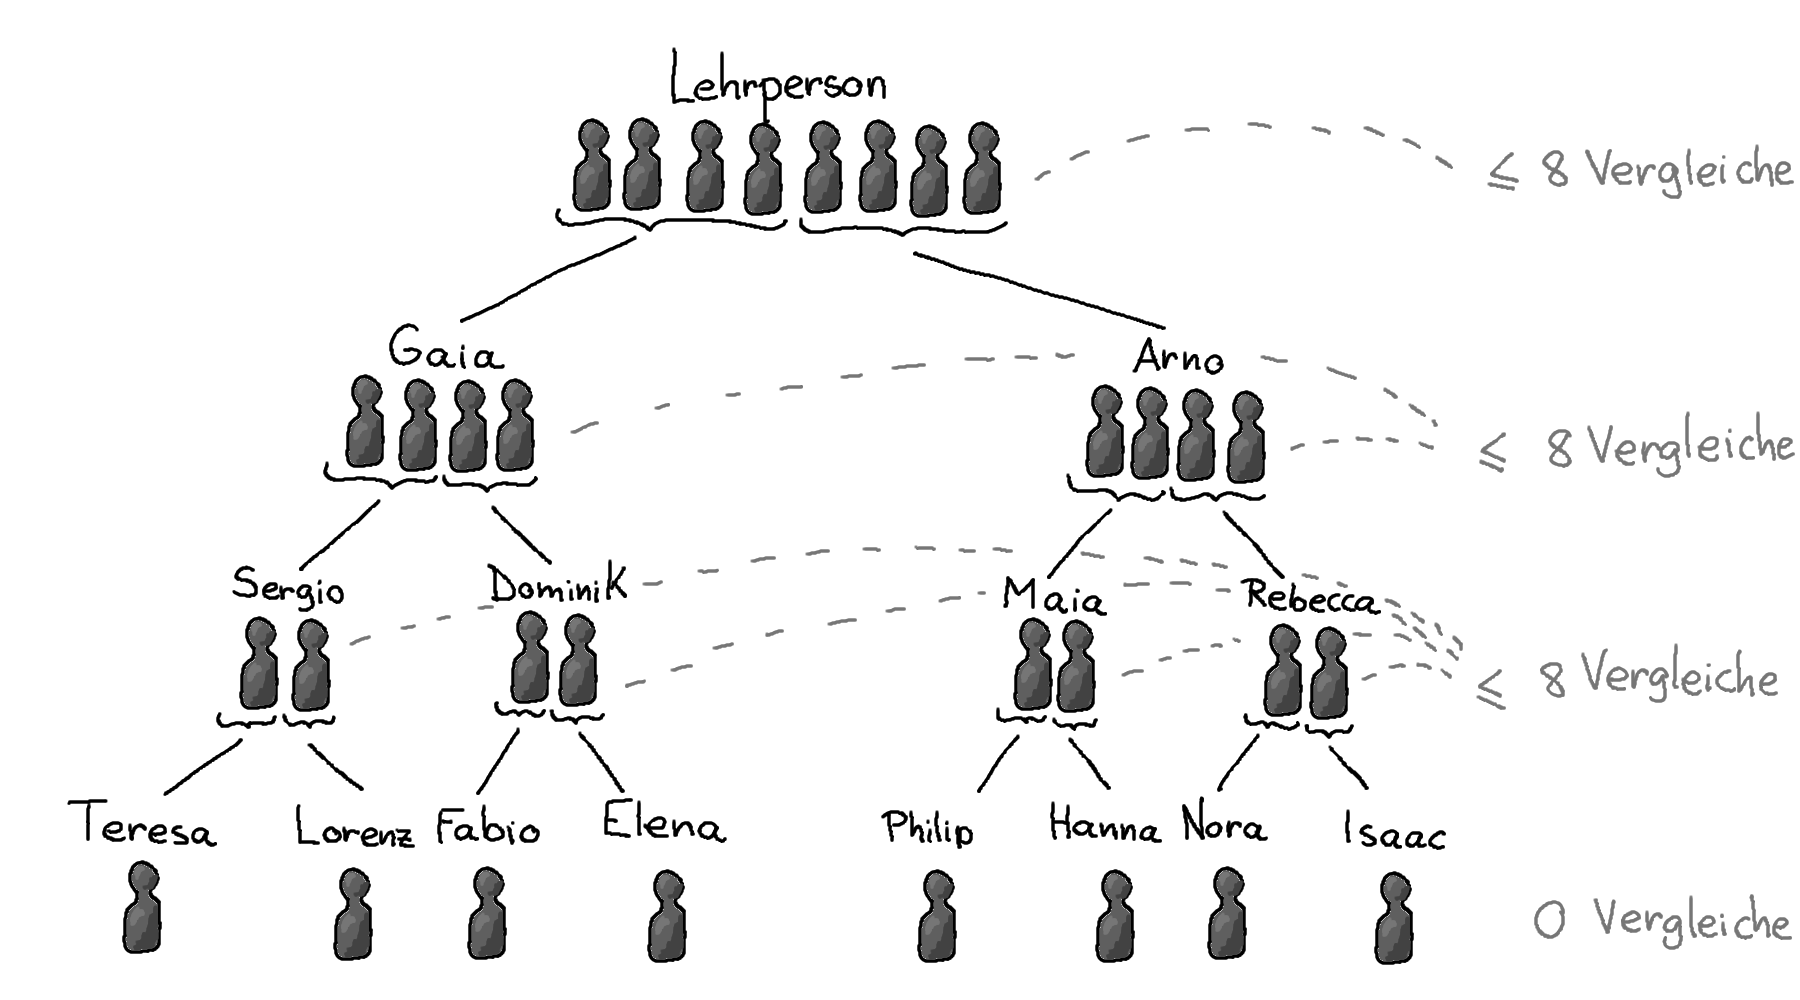
\includegraphics[width=\textwidth]{Mergesort_Aktivitaet.png}
	\caption{Mergesort wird von der Klasse ausgeführt. Die Lehrperson hat 8 Gewichter. Sie gibt je 4 davon einem SuS zum sortieren und fügt nachher die sortierten Teile zusammen. Um zwei sortierte Teillisten zusammenzufügen braucht die Lehrperson höchstens 8 Vergleiche. Die SuS verwenden das gleiche Verfahren, um ihre kleinere Listen zu sortieren: sie ''outsourcen'' das Sortieren der Teillisten und übernehmen nur das Zusammenfügen der sortierten Teillisten. Schüler, die nur ein Gewicht erhalten, müssen ihre Liste selber sortieren. In dieser Baumdarstellung sieht man, dass die Anzahl der benötigten Vergleiche höchstens \(8 \cdot log(8)\) ist.}
\end{figure}

Nach der Aktivität können die SuS eine Schätzung angeben, wie viele Vergleiche würden sie mit 16 oder 32 Gewichter brauchen.

Anschliessend analysiert man in Plenum, wie sich die Anzahl der benötigten Vergleiche abhängig von der Anzahl der Gewichter entwickelt. An der Tafel mit dem Baumdiagramm wird erklärt, dass die Anzahl der Vergleiche im Allgemeinen höchstens \(n \cdot log(n)\) ist. Dasselbe wird auch mathematisch mit der rekursiven Laufzeitfunktion berechnet: \(T(n) \leq T(n/2) + T(n/2) + n - 1\) mit \(T(1) = 0\). Es wird nicht genau \(T(n)\) berechnet, sondern eine obere Schranke dafür. Nun soll man das mit den Algorithmen aus der ersten Doppellektion vergleichen und sehen, dass es Algorithmen existieren, die dasselbe machen, aber wesentlich schneller sind, als andere.

Falls die Klasse programmiert, kann man ihnen zwei Implementierungen zweier Sortieralgorithmen geben, z.B. Sortieren durch Auswählen und Mergesort, die sie benchmarken und plotten sollen, um sich davon zu überzeugen, dass die theoretisch berechnete Anzahl Vergleiche tatsächliche Auswirkungen auf die Laufzeit von Programmen hat.

\section*{Bezug zur Allgemeinbildung}
Auch wenn Sortieren und Suchen immer mehr vom Rechner übernommen werden und scheinbar gar keine Zeit brauchen, ist es dennoch wichtig zu wissen, dass dahinter mehr oder weniger effiziente Algorithmen stehen. Bei der immer steigenden Datenmenge und ungefähr gleich bleibender Prozessorgeschwindigkeit werden wir wahrscheinlich bald wieder die Vor- und Nachteile von Sortieren beobachten können.

Die Konzepte von Rekursion und ''Teilen und Herrschen'', die  am Beispiel von Mergesort veranschaulicht wurden, lassen sich in der Algorithmenentwicklung auch für andere Probleme anwenden. Ausserdem, bekommen die SuS ein Instrument, um verschiedene Algorithmen, die das gleiche Problem lösen, bezüglich ihrer Laufzeit miteinander zu vergleichen.


\section*{Eignung für die Altersstufe}
Der vorgeschlagene Ansatz fördert Kompetenzen, die die SuS vor einem Studium an einer Hochschule erwerben sollten. Einerseits stärkt das mathematische Kompetenzen, Abhängigkeiten zwischen Grössen als Funktionen aufzufassen, und Problemlösungsfähigkeiten, da die SuS selbstständig einen Sortieralgorithmus entwickeln müssen. Anderseits fördert dieses Vorgehen sprachliche Kompetenzen, eigene Ideen und Verfahren verständlich für andere auszudrücken, und stärkt die Teamfähigkeit.

Der Bezug auf greifbare physikalische Gegenstände wie Waage und Gewichter schlägt eine Brücke zwischen der echten Welt, die wir mit unseren Sinnen beobachten, und der digitalen Magie, die angeblich im Inneren von einem Computer abläuft.


\end{document}
